\documentclass[11pt,a4paper]{article}

% --- Core Packages ---
\usepackage[utf8]{inputenc}
\usepackage[T1]{fontenc}
\usepackage{amsmath, amssymb, amsfonts, amsthm}
\usepackage{geometry}
\usepackage{xcolor}
\usepackage{graphicx}
\usepackage{booktabs}
\usepackage{array}
\usepackage{enumitem}
\usepackage{fancyhdr}
\usepackage{sectsty}
\usepackage[colorlinks=true, linkcolor=RoyalBlue, citecolor=RoyalBlue, urlcolor=RoyalBlue]{hyperref}

% --- TikZ Setup for Diagrams ---
\usepackage{tikz}
\usetikzlibrary{arrows.meta, positioning, calc}

% --- Elegant Styling & Boxes ---
\usepackage[most]{tcolorbox}

% Define Theme Colors
\definecolor{RoyalBlue}{rgb}{0.08, 0.35, 0.65}
\definecolor{DarkSlate}{rgb}{0.15, 0.20, 0.25}
\definecolor{CrimsonRed}{rgb}{0.75, 0.10, 0.15}
\definecolor{ForestGreen}{rgb}{0.10, 0.55, 0.20}
\definecolor{Eggplant}{rgb}{0.38, 0.12, 0.38}
\definecolor{SoftGray}{rgb}{0.96, 0.97, 0.98}
\definecolor{dimgray}{rgb}{0.41, 0.41, 0.41}

% Apply Margins
\geometry{
    top=1.0in,
    bottom=1.0in,
    left=0.85in,
    right=0.85in,
    headheight=14pt
}

% Section and Subsection Fonts
\sectionfont{\color{RoyalBlue}\sectionrule{0pt}{0pt}{-5pt}{1pt}}
\subsectionfont{\color{Eggplant}}
\subsubsectionfont{\color{DarkSlate}}

% Headers and Footers
\pagestyle{fancy}
\fancyhf{}
\fancyhead[L]{\color{gray}\itshape Electricity \& Magnetism --- Past Year Practice Questions}
\fancyhead[R]{\color{gray}\itshape Revision Guide}
\fancyfoot[C]{\thepage}
\renewcommand{\headrulewidth}{0.4pt}

% --- Styled Custom TColorBoxes ---
\newtcolorbox{questionbox}[1][]{
    enhanced,
    colback=white,
    colframe=RoyalBlue,
    width=\textwidth,
    arc=2mm,
    boxrule=1.2pt,
    title=\textbf{#1},
    coltitle=white,
    colbacktitle=RoyalBlue,
    attach boxed title to top left={yshift=-2mm, xshift=5mm},
    boxed title style={arc=1mm},
    fonttitle=\sffamily\bfseries\small,
    drop shadow={RoyalBlue!15!white}
}

\newtcolorbox{solutionbox}[1][]{
    enhanced,
    colback=ForestGreen!3!white,
    colframe=ForestGreen,
    width=\textwidth,
    arc=2mm,
    boxrule=1.2pt,
    title=\textbf{#1},
    coltitle=white,
    colbacktitle=ForestGreen,
    attach boxed title to top left={yshift=-2mm, xshift=5mm},
    boxed title style={arc=1mm},
    fonttitle=\sffamily\bfseries\small,
    drop shadow={ForestGreen!10!white}
}

\newtcolorbox{prioritybox}[1][]{
    enhanced,
    colback=RoyalBlue!5!white,
    colframe=RoyalBlue!80!black,
    width=\textwidth,
    arc=3mm,
    boxrule=1.5pt,
    title=\textbf{#1},
    coltitle=white,
    colbacktitle=RoyalBlue!80!black,
    attach boxed title to top left={yshift=-2.5mm, xshift=5mm},
    boxed title style={arc=1.5mm},
    fonttitle=\sffamily\bfseries,
    drop shadow={RoyalBlue!15!white}
}

\begin{document}

% --- Cover Title ---
\begin{center}
    \vspace*{1cm}
    {\Huge\bfseries\color{RoyalBlue} Electricity \& Magnetism}\\[0.4cm]
    {\Large\bfseries\color{Eggplant} Past Year Practice Questions (PYQ-Oriented)}\\[0.6cm]
    \rule{\linewidth}{1.5pt}\\[1.0cm]
\end{center}

\section{Introduction}
This workbook contains a curated collection of high-weightage conceptual, numerical, and derivation-based practice questions. These are selected directly from university past year papers (PYQs) to test your conceptual understanding, problem-solving skills, and preparation readiness.

\newpage
% =========================================================================
% PART A: CONCEPTUAL QUESTIONS
% =========================================================================
\section{Part A: Conceptual High-Yield Questions}

\begin{questionbox}[Question 1: Electric Field Lines]
    Explain why two electric field lines can never intersect each other.
\end{questionbox}

\begin{solutionbox}[Detailed Solution]
    Electric field lines represent the path that a positive test charge would naturally follow in an electric field. The tangent to a field line at any given point gives the direction of the net electric field vector $\vec{E}$ at that point.
    
    If two field lines were to intersect at a point $X$, it would imply that at this single point of intersection, we could draw two unique tangents. This means the net electric field $\vec{E}$ would point in \textbf{two different directions simultaneously} at the same location:
    \begin{center}
        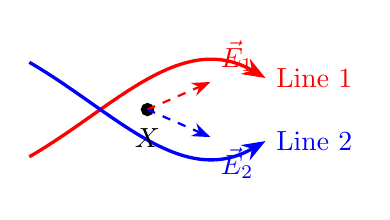
\begin{tikzpicture}[>=Stealth, thick]
            \draw [red, ->, very thick] (0,0) to [out=30, in=150] (3,1) node[right] {Line 1};
            \draw [blue, ->, very thick] (0,1.2) to [out=-30, in=-150] (3,0.2) node[right] {Line 2};
            \filldraw [black] (1.5, 0.6) circle (2pt) node[below=3pt] {$X$};
            \draw [->, red, dashed, thick] (1.5,0.6) -- (2.3, 0.95) node[above right] {$\vec{E}_1$};
            \draw [->, blue, dashed, thick] (1.5,0.6) -- (2.3, 0.25) node[below right] {$\vec{E}_2$};
        \end{tikzpicture}
    \end{center}
    Since the electric field vector at any point must be unique, this is physically impossible. Therefore, two electric field lines can never cross or intersect.
\end{solutionbox}

\vspace{0.8cm}

\begin{questionbox}[Question 2: Temperature Dependence of Magnetism]
    Explain the difference in temperature dependence of magnetic susceptibility between diamagnetic and paramagnetic materials.
\end{questionbox}

\begin{solutionbox}[Detailed Solution]
    The physical mechanisms driving diamagnetism and paramagnetism are fundamentally different:
    \begin{enumerate}
        \item \textbf{Diamagnetic Materials:} Diamagnetism arises from the induced orbital motion of electrons in response to an external magnetic field (Lenz's Law on an atomic scale). Since this is an orbital effect inherent to the electron shells, it is completely unaffected by thermal agitation. Therefore, the magnetic susceptibility $\chi_d$ of a diamagnetic substance is \textbf{independent of temperature}.
        \item \textbf{Paramagnetic Materials:} Paramagnetism arises from the alignment of permanent atomic magnetic dipoles. At higher temperatures, thermal agitation randomizes the dipole orientations, opposing the alignment. Thus, paramagnetic susceptibility $\chi_p$ is inversely proportional to the absolute temperature $T$. This behavior is described by \textbf{Curie's Law}:
        \[ \chi_p = \frac{C}{T} \]
        Where $C$ is the Curie constant.
    \end{enumerate}
\end{solutionbox}

\newpage
% =========================================================================
% PART B: NUMERICAL PROBLEMS
% =========================================================================
\section{Part B: Numerical Problems (With Steps)}

\begin{questionbox}[Problem 1: Electric Potential at Center of Square]
    Four point charges $q_1 = 1 \times 10^{-8}\text{ C}$, $q_2 = -2 \times 10^{-8}\text{ C}$, $q_3 = 3 \times 10^{-8}\text{ C}$, and $q_4 = 2 \times 10^{-8}\text{ C}$ are placed at the four corners of a square of side $1.0\text{ m}$. Calculate the electric potential at the center of the square. *(DU Set 2 PYQ)*
\end{questionbox}

\begin{solutionbox}[Step-by-Step Solution]
    \textbf{Step 1: Determine the distance of each corner from the center ($r$).}
    For a square of side $a = 1.0\text{ m}$, the length of the diagonal is:
    \[ d = a\sqrt{2} = 1.0\sqrt{2}\text{ m} \]
    The distance from each corner to the center of the square is half the diagonal:
    \[ r = \frac{d}{2} = \frac{\sqrt{2}}{2} = \frac{1}{\sqrt{2}} \approx 0.707\text{ m} \]
    
    \textbf{Step 2: Use the Superposition Principle for Potential.}
    Since electric potential is a scalar quantity, the total potential $V$ at the center is the algebraic sum of the potentials produced by the four charges:
    \[ V = \frac{1}{4\pi\epsilon_0} \frac{q_1 + q_2 + q_3 + q_4}{r} \]
    
    \textbf{Step 3: Calculate the total net charge.}
    \[ \sum q = q_1 + q_2 + q_3 + q_4 = (1 - 2 + 3 + 2) \times 10^{-8}\text{ C} = 4 \times 10^{-8}\text{ C} \]
    
    \textbf{Step 4: Substitute the numerical values.}
    Using $\frac{1}{4\pi\epsilon_0} = 9 \times 10^9 \text{ N}\cdot\text{m}^2/\text{C}^2$:
    \[ V = 9 \times 10^9 \times \frac{4 \times 10^{-8}}{0.707} = \frac{360}{0.707} \approx 509.2\text{ V} \]
    
    \textbf{Answer:} The electric potential at the center of the square is approximately \textbf{509.2 Volts}.
\end{solutionbox}

\vspace{0.8cm}

\begin{questionbox}[Problem 2: Solenoid with Magnetic Core]
    A long solenoid is wound with 10 turns per centimeter and carries a current of $2.0\text{ A}$. If a magnetic core with relative permeability $\mu_r = 400$ is placed inside the solenoid, calculate the magnetic field $B$ inside the core. *(DU Set 3 PYQ)*
\end{questionbox}

\begin{solutionbox}[Step-by-Step Solution]
    \textbf{Step 1: Convert turns per unit length to standard SI units ($n$).}
    Given $n = 10 \text{ turns/cm}$. Converting to turns per meter:
    \[ n = 10 \text{ turns/cm} \times 100 \text{ cm/m} = 1000 \text{ turns/m} \]
    
    \textbf{Step 2: Write the magnetic field formula with relative permeability.}
    For a solenoid containing a magnetic core:
    \[ B = \mu n I = \mu_0 \mu_r n I \]
    
    \textbf{Step 3: Substitute the known constants and values.}
    * Permeability of free space: $\mu_0 = 4\pi \times 10^{-7}\text{ T}\cdot\text{m/A}$
    * Relative permeability: $\mu_r = 400$
    * Current: $I = 2.0\text{ A}$
    * Turns per meter: $n = 1000\text{ m}^{-1}$
    
    \[ B = (4\pi \times 10^{-7}) \times 400 \times 1000 \times 2.0 \]
    \[ B = 4\pi \times 10^{-7} \times 8 \times 10^5 = 32\pi \times 10^{-2}\text{ T} \]
    \[ B = 0.32\pi \approx 1.005\text{ T} \]
    
    \textbf{Answer:} The magnetic field inside the magnetic core is approximately \textbf{1.01 Tesla}.
\end{solutionbox}

\newpage
% =========================================================================
% PART C: HIGH-YIELD DERIVATION CHECKLISTS
% =========================================================================
\section{Part C: High-Yield Derivation Exam Checklists}

\begin{prioritybox}[Derivation 1: Electric Potential of a Dipole]
    \textbf{Goal:} Derive $V = \frac{1}{4\pi\epsilon_0}\frac{p\cos\theta}{r^2}$ for $r \gg a$.
    \begin{itemize}
        \item[\textbf{1.}] **Geometry Setup:** Draw a dipole along the x-axis from $-q$ at $(-a,0)$ to $+q$ at $(a,0)$. Define a target point $P(r,\theta)$ relative to the center $O$.
        \item[\textbf{2.}] **Algebraic Equations:** Write the potential equations:
        \[ V = \frac{q}{4\pi\epsilon_0} \left( \frac{1}{r_+} - \frac{1}{r_-} \right) \]
        \item[\textbf{3.}] **Binomial Approximations:** Express distances $r_+$ and $r_-$ from the charges:
        \[ r_+ = r(1 - \frac{a}{r}\cos\theta) \quad \implies \quad \frac{1}{r_+} \approx \frac{1}{r}(1 + \frac{a}{r}\cos\theta) \]
        \[ r_- = r(1 + \frac{a}{r}\cos\theta) \quad \implies \quad \frac{1}{r_-} \approx \frac{1}{r}(1 - \frac{a}{r}\cos\theta) \]
        \item[\textbf{4.}] **Final Step:** Substitute the approximations and use $p = 2aq$ to obtain the final formula.
    \end{itemize}
\end{prioritybox}

\vspace{0.8cm}

\begin{prioritybox}[Derivation 2: Maximum Power Transfer Theorem]
    \textbf{Goal:} Prove $R_L = R_{\text{th}}$ for maximum load power.
    \begin{itemize}
        \item[\textbf{1.}] **Circuit Representation:** Draw a series circuit with a Thevenin source $V_{\text{th}}$, internal resistance $R_{\text{th}}$, and adjustable load $R_L$.
        \item[\textbf{2.}] **Power Equation:** Formulate load power:
        \[ P_L = I^2 R_L = \left( \frac{V_{\text{th}}}{R_{\text{th}} + R_L} \right)^2 R_L \]
        \item[\textbf{3.}] **Maximization Condition:** Differentiate $P_L$ using the quotient rule:
        \[ \frac{dP_L}{dR_L} = 0 \quad \implies \quad (R_{\text{th}} + R_L)^2 - 2R_L(R_{\text{th}} + R_L) = 0 \]
        \item[\textbf{4.}] **Efficiency Verification:** Solve to find $R_L = R_{\text{th}}$. Show that under this condition, the maximum power is $P_{\text{max}} = \frac{V_{\text{th}}^2}{4R_{\text{th}}}$, and the efficiency $\eta = 50\%$.
    \end{itemize}
\end{prioritybox}

\end{document}
